%% inst.tex %%
\begin{frame}
 \frametitle{Graphe critique pour les algorithmes d'approximation}
 
 \begin{block}{Données}
  \begin{center}
   \begin{figure}[!ht]
    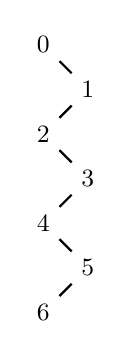
\begin{tikzpicture}[font=\small]
     \tikzstyle{level 1}=[level distance=0.8cm, sibling distance=0.8cm]
     \tikzstyle{childnode}=[rounded corners]
     \tikzstyle{marknode}=[fill=red!30, rounded corners]
     \tikzstyle{edge from parent}=[draw,thick]
     \node[childnode] {0} 
      child[grow=south east] {node[childnode] {1} 
       child[grow=south west] {node[childnode] {2}
        child[grow=south east] {node[childnode] {3}
         child[grow=south west] {node[childnode] {4}
          child[grow=south east] {node[childnode] {5}
           child[grow=south west] {node[childnode] {6} 
           }
          }
         }
        }
       }
      };
    \end{tikzpicture}

    \caption{Graphe \emph{serpent}}
   \end{figure}
  \end{center}
 \end{block}
\end{frame}

\begin{frame}
 \frametitle{Solution pour le graphe \emph{serpent}}

 \begin{center}
  \begin{block}{Comparaison des solutions sur le graphe \emph{serpent}}
   \begin{figure}[!ht]
    \setlength{\tabcolsep}{1cm}
    \begin{tabular}{cc}
     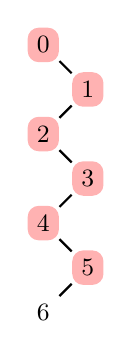
\begin{tikzpicture}[font=\small]
      \tikzstyle{level 1}=[level distance=0.8cm, sibling distance=0.8cm]
      \tikzstyle{childnode}=[rounded corners]
      \tikzstyle{marknode}=[fill=red!30, rounded corners]
      \tikzstyle{edge from parent}=[draw,thick]
      \node[marknode] {0} 
       child[grow=south east] {node[marknode] {1} 
        child[grow=south west] {node[marknode] {2}
         child[grow=south east] {node[marknode] {3}
          child[grow=south west] {node[marknode] {4}
           child[grow=south east] {node[marknode] {5}
            child[grow=south west] {node[childnode] {6} 
           }
          }
         }
        }
       }
      };
     \end{tikzpicture}
     &
     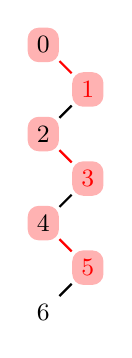
\begin{tikzpicture}[font=\small]
      \tikzstyle{level 1}=[level distance=0.8cm, sibling distance=0.8cm]
      \tikzstyle{childnode}=[rounded corners]
      \tikzstyle{marknode}=[fill=red!30, rounded corners]
      \tikzstyle{edge from parent}=[draw,thick]
      \node[marknode] {0} 
       child[grow=south east, red] {node[marknode] {\Cb{1}} 
        child[grow=south west, black] {node[marknode] {2}
         child[grow=south east, red] {node[marknode] {\Cb{3}}
          child[grow=south west, black] {node[marknode] {4}
           child[grow=south east, red] {node[marknode] {\Cb{5}}
            child[grow=south west, black] {node[childnode] {6} 
            }
           }
          }
         }
        }
       };
     \end{tikzpicture}\\
     $C_{projet} = \{0,1,2,3,4,5\}$ & $C_{cours} = \{0,1,2,3,4,5\}$\\
    \end{tabular}
   \end{figure}    
  \end{block}
 \end{center}
\end{frame}

\begin{frame}
 \frametitle{Graphe critique pour les algorithmes d'approximation}
 
 \begin{block}{Couverture minimale surle graphe \emph{serpent}}
  \begin{center}
   \begin{figure}[!ht]
    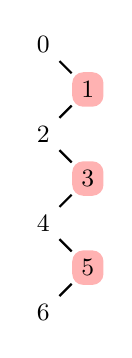
\begin{tikzpicture}[font=\small]
     \tikzstyle{level 1}=[level distance=0.8cm, sibling distance=0.8cm]
     \tikzstyle{childnode}=[rounded corners]
     \tikzstyle{marknode}=[fill=red!30, rounded corners]
     \tikzstyle{edge from parent}=[draw,thick]
     \node[childnode] {0} 
      child[grow=south east] {node[marknode] {1} 
       child[grow=south west] {node[childnode] {2}
        child[grow=south east] {node[marknode] {3}
         child[grow=south west] {node[childnode] {4}
          child[grow=south east] {node[marknode] {5}
           child[grow=south west] {node[childnode] {6} 
           }
          }
         }
        }
       }
      };
    \end{tikzpicture}
   \end{figure}
   Couverture minimale = $\{1,3,5\}$
  \end{center}
 \end{block}
\end{frame}
